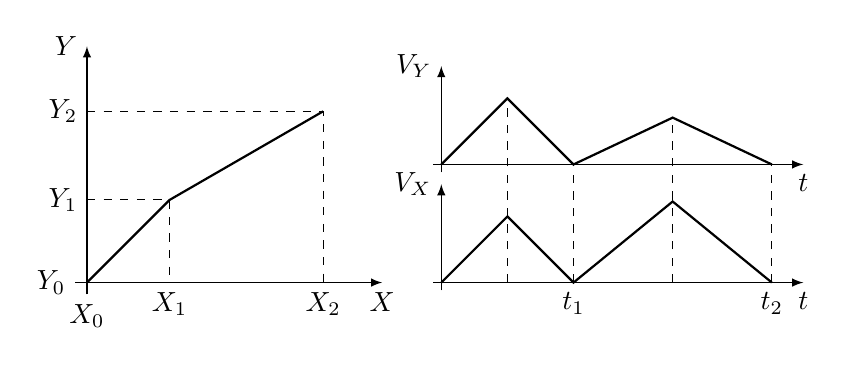
\begin{tikzpicture}
%
%Positionen/Kontur
%
\begin{scope}[xscale = 0.15,yscale = 0.15]
%
\draw[-latex] (-1,0)node[left]{$Y_0$}--(25,0)node[below]{$X$};
\draw[-latex] (0,-1)node[below]{$X_0$}--(0,20)node[left]{$Y$};
%
\draw[thick](0,0)--(7,7)--(20,14.5);
%
\draw[dashed](0,7)node[left]{$Y_1$}--(7,7)--(7,0)node[below]{$X_1$};
\draw[dashed](0,14.5)node[left]{$Y_2$}--(20,14.5)--(20,0)node[below]{$X_2$};
%
\end{scope}
%
\begin{scope}[xshift = 4.5cm,xscale = 0.01,yscale = 0.01]
%
\draw[-latex] (-10,0)--(460,0)node[below]{$t$};
\draw[-latex] (0,-10)--(0,125)node[left]{$V_X$};
%
\draw[thick](0,0)--(84,84)--(168,0)node[below]{$t_1$}--(294,103)--(420,0)node[below]{$t_2$};
%
\draw[dashed](84,0)--(84,230);
\draw[dashed](168,0)--(168,150);
\draw[dashed](294,0)--(294,200);
\draw[dashed](420,0)--(420,150);
%
\end{scope}
%
\begin{scope}[xshift = 4.5cm,yshift = 1.5cm,xscale = 0.01,yscale = 0.01]
%
\draw[-latex] (-10,0)--(460,0)node[below]{$t$};
\draw[-latex] (0,-10)--(0,125)node[left]{$V_Y$};
%
\draw[thick](0,0)--(84,84)--(168,0)--(294,59.5)--(420,0);
%
\end{scope}
%
\end{tikzpicture}